\documentclass[11pt,a4paper]{article}

\usepackage[margin=2.5cm]{geometry}
\usepackage{booktabs}
\usepackage{array}
\usepackage{tabularx}
\usepackage{longtable}
\usepackage{hyperref}
\usepackage{placeins}
\usepackage{amsmath,amssymb}
\usepackage{graphicx}
\usepackage{xcolor}
\usepackage{enumitem}
\usepackage{microtype}

\definecolor{navy}{HTML}{24466F}
\definecolor{teal}{HTML}{2F7D68}
\definecolor{lightblue}{HTML}{EEF4FA}
\definecolor{lightgray}{HTML}{F4F5F7}
\hypersetup{
    colorlinks=true,
    linkcolor=navy,
    urlcolor=teal,
    citecolor=navy
}
\setlist{nosep,leftmargin=*}
\renewcommand{\arraystretch}{1.15}

\title{\textbf{Concept-Guided Mitigation of Spurious Correlations in Self-Supervised Representations}\\[0.4em]
\large Progress report for supervisor meeting}
\author{Grigory Grechkin}
\date{21 July 2026}

\begin{document}
\maketitle

\begin{center}
\fcolorbox{navy}{lightblue}{
\begin{minipage}{0.91\textwidth}
\textbf{Executive result.}
I built a reproducible pipeline that uses a frozen, interpretable SpLiCE model
to discover possible background concepts and to guide SimCLR training. The
current post-repair experiments do \emph{not} show a reliable worst-group (WG)
improvement over matched SimCLR. The strongest completed revised setting,
correlation regularization with $\lambda=0.1$, reaches
$48.49\pm4.37\%$ WG accuracy versus $48.04\pm2.82\%$ for SimCLR
($+0.45$ points on average), but the paired seed effects are
$+2.38,+6.27,-7.30$ points. This is therefore a diagnostic result, not evidence
of a robust gain. The most promising next step is to improve concept selection
and use the concepts to construct cross-background positive pairs directly
inside the contrastive objective.
\end{minipage}}
\end{center}

\section{Research Question and Current Answer}

This project tests the hypothesis that concept-level information from a frozen
vision--language model can identify and weaken shortcut information learned by a
self-supervised encoder. SpLiCE is used to discover concepts associated with the
known spurious attribute after conditioning on the target label. The resulting
signal is then used in three distinct ways: (i) as an audit of dataset bias,
(ii) as guidance for SimCLR training through targeted augmentation or a
label-conditioned correlation regularizer, and (iii) as a direct sparse
SpLiCE concept-bottleneck (CBM) intervention baseline. The trained SSL encoder
remains a ResNet; the CLIP/SpLiCE model is frozen.

The central empirical prediction is not merely an increase in average accuracy.
If the intervention reduces shortcut reliance, worst-group (WG) validation and
test accuracy should improve relative to a matched SimCLR baseline, while a
probe trained to predict the spurious attribute should become less successful.
All hyperparameter selection is performed on validation data and the test split
is reserved for a final, preselected configuration.

\begin{table}[ht]
\centering
\caption{At-a-glance status for the meeting.}
\begin{tabularx}{\textwidth}{>{\bfseries}p{0.25\textwidth} X}
\toprule
Question & Current answer \\
\midrule
What was built? & End-to-end concept discovery, cached SpLiCE scoring,
concept-guided augmentation, conditional correlation regularization, periodic
target and leakage probes, guarded test evaluation, and reproducible Slurm/W\&B
experiment arrays. \\
What is the main result? & The revised automatic methods have not yet produced
a stable WG improvement across comparable seeds. REG $\lambda=0.1$ is the only
completed setting above baseline in the three-seed mean, and only by 0.45 points. \\
What did we learn? & The intervention effect is strongly seed-dependent; the
small REG weight was effectively negligible; aggressive routed augmentation can
make optimization harder; and the current automatic concept set is not purely
background-specific. \\
What should happen next? & Audit concept direction and specificity, add shuffled
and random-routing controls, then test concept-conditioned cross-background
contrastive positives before spending compute on more seeds or final test runs. \\
\bottomrule
\end{tabularx}
\end{table}

\section{What Is Linear, and What Is Already Contrastive?}

SpLiCE is \emph{not} the classifier trained in the main experiments. It is a
post-hoc sparse coding method: a frozen CLIP image embedding is approximated by
a nonnegative linear combination of frozen text-concept embeddings, with an
$\ell_1$ penalty encouraging a short explanation \cite{bhalla2024splice}. The
word ``linear'' therefore describes the concept decomposition, not the full
vision system.

The complete pipeline contains four different objects:
\begin{enumerate}
    \item \textbf{Frozen CLIP encoder:} a nonlinear vision transformer that
    produces the dense embedding which SpLiCE explains.
    \item \textbf{SpLiCE decomposition:} a sparse nonnegative linear
    reconstruction of that embedding in a text-concept dictionary.
    \item \textbf{Trainable SSL encoder:} a nonlinear ResNet18 trained from
    scratch in this project.
    \item \textbf{Linear probe:} a linear classifier trained only after SSL to
    measure what information is linearly accessible in the representation.
\end{enumerate}

The main SSL loss is already contrastive: the implementation uses the SimCLR
NT-Xent/InfoNCE objective on two augmented views of each image
\cite{chen2020simclr}. Consequently, ``try a contrastive objective'' is not an
alternative to the current setup. The useful question is whether to make the
\emph{pair construction or weighting} concept-aware, or whether to add a
better-scaled invariance objective to the existing contrastive loss.

\section{Brief Description of SpLiCE}

SpLiCE, Sparse Linear Concept Embeddings, decomposes dense CLIP image embeddings
into sparse nonnegative weights over a vocabulary of human-interpretable text
concepts. Instead of treating a CLIP image feature as an opaque vector, SpLiCE
approximates it as a linear combination of text-concept embeddings. This makes
it possible to assign each image a score for selected concepts, such as concepts
related to the Waterbirds background. In this project SpLiCE is a frozen helper
model used for auditing and control, not the SSL encoder being trained and not a
replacement for the ResNet classifier.

The current configuration uses an \texttt{open\_clip:ViT-B-32} backbone with
\texttt{laion2b\_s34b\_b79k} weights, the LAION vocabulary of size 10\,000, and
an $\ell_1$ penalty of 0.25. SpLiCE returns a sparse nonnegative concept vector.
After automatic dataset-level selection of ten coordinates, their full
per-image vector is retained for regularization. A scalar maximum is used only
for routing images to the strong-augmentation branch. The augmentation and
correlation objectives are extensions developed in this project rather than
methods claimed by the original SpLiCE paper; the sparse CBM intervention is
the closest direct analogue of concept-space editing.

\section{Concrete Contributions Over the Last Weeks}

\begin{table}[ht]
\centering
\caption{Implemented work and why it matters scientifically.}
\begin{tabularx}{\textwidth}{>{\bfseries}p{0.20\textwidth} X X}
\toprule
Workstream & Implementation & Scientific value \\
\midrule
Bias discovery & Dataset-level conditional ranking of SpLiCE concepts using
target and background metadata; shared cached top-$K$ vectors. & Turns a vague
idea (``find background concepts'') into a reproducible, inspectable signal. \\
Training interventions & Concept-routed strong augmentation and a
target-conditioned feature--concept correlation penalty. & Tests two distinct
mechanisms: invariance through views and information removal through a loss. \\
Evaluation & Periodic balanced linear probes, WG metrics, optional spurious
attribute probe, and a final-test guard. & Separates average performance from
minority-group robustness and reduces test-selection leakage. \\
Reproducibility & Isolated diagnostic loaders, restored RNG states, deterministic
paired runs, checkpoint state, W\&B tags/groups, and array-safe concept discovery. &
Made it possible to discover that the initially positive result did not
replicate under the repaired protocol. \\
Baselines and scope & Sparse SpLiCE-CBM intervention, component ablations,
Waterbirds/SpurCIFAR10/CelebA-compatible data paths, and tests. & Supports both
mechanistic diagnosis and later transfer beyond one dataset. \\
\bottomrule
\end{tabularx}
\end{table}

\section{Implementation in This Repository}

The original SpLiCE package is kept in \texttt{splice/}. The project-specific
integration is implemented mainly in \texttt{spur\_splice.py},
\texttt{splice/ssl\_regularization.py}, and the Waterbirds dataset utilities in
\texttt{experiments/spurious\_eval/}. The entry point \texttt{spur\_splice.py}
runs SimCLR training, checkpointing, optional periodic linear probing, and
logging. SpLiCE is enabled through \texttt{--splice\_mode}, with supported modes
\texttt{none}, \texttt{augment}, \texttt{corr\_reg}, and
\texttt{augment\_corr\_reg}.

\subsection{Workflow}

\begin{enumerate}

    \item If a SpLiCE mode is enabled, the training split is decomposed once by
    a frozen SpLiCE model. Concepts are ranked using target- and spurious-group
    metadata, and the shared dataset-level top-10 is cached. For example, for the
    Waterbirds runs this set is \texttt{bamboo, forests, whale, rainforest,
    raven, forest, seascape, lake, snorkeling, pond}.

    \item The Waterbirds SSL dataset wraps the usual WILDS-style subset with
    the cached selected-concept vectors. Each item returns two SimCLR views,
    the label, metadata, and a vector $c(x)\in\mathbb{R}^{10}_{\geq 0}$.

    \item In \texttt{augment} mode, $r(x)=\max_k c_k(x)$ controls routing. The
    threshold is a quantile computed on the training split. A high-score image produces the pair
    $[T_{\mathrm{std}}(x),T_{\mathrm{strong}}(x)]$; a low-score image produces
    two standard views. This gives SimCLR an explicit invariance pair without
    corrupting both views with the strong transform.

    \item In \texttt{corr\_reg} mode, the loss penalizes the complete matrix of
    correlations between SSL dimensions and the ten selected concepts. Both
    representations are centred within each target class before correlations
    are computed. This label-conditioned formulation avoids penalizing useful
    target information merely because target and background are correlated in
    the biased training split.

    \item Linear probing is decoupled from checkpoint retention and is run every
    25 SSL epochs during validation development. The target probe is trained on
    the balanced \texttt{ds\_train} split and evaluated on \texttt{val}. A
    \texttt{--final\_test} mode performs one final test probe only after model
    and hyperparameters have been fixed.
\end{enumerate}

\section{Supporting Tools}

Utility scripts and caches were added to make the SpLiCE configuration reproducible.
\texttt{tools/
discover\_splice\_spurious\_concepts.py} decomposes images by
metadata group and ranks concepts by how strongly they vary with the spurious
attribute while penalizing class-label effects. This helps choose candidate
background concepts. \texttt{tools/summarize\_splice\_scores.py} reports the
distribution of selected concept scores. A sparse SpLiCE-CBM entry point and optional
representation/probe interventions were also added.

The implementation was repaired so that rank diagnostics and periodic probes
do not advance the SSL data-loader random state. Seeds 1, 3, and 4 form the
current comparable post-repair set; seeds 0 and 2 are retained only as
historical descriptive points. This distinction is central to the interpretation
below.

\section{Experimental Protocol}

The primary revised comparison uses post-repair seeds 1, 3, and 4. The
augmentation sweep varies the train-score quantile $q$; the regularization sweep
varies $\lambda$. The augmentation-component array keeps $q=0.75$ and changes
only the strong transform. Runs are compared using the mean of the final ten
periodic validation probes at SSL epoch 1000; per-run peak epochs are not used
for selection. Seeds 0 and 2 predate the reproducibility repair and are shown
only to make the experimental history transparent.

\begin{table}[h]
\centering
\caption{Fixed experiment settings}
\begin{tabularx}{\textwidth}{>{\bfseries}l X}
\toprule
Setting & Value \\
\midrule
Dataset & Waterbirds \\
SSL method & SimCLR \\
SSL encoder & \texttt{ResNet18-large} \\
SpLiCE model & \texttt{open\_clip:ViT-B-32}, \texttt{laion2b\_s34b\_b79k} \\
Vocabulary & \texttt{LAION}, size 10\,000 \\
Selected Top-10 SpLiCE concepts & bamboo,forests,whale,rainforest,raven,forest,seascape,
lake,snorkeling,pond \\
SpLiCE routing & maximum over selected vector; train quantile $q$ \\
Linear-probe train split & \texttt{ds\_train} (group-balanced) \\
Batch size & 256 \\
Learning rate & 0.01 \\
Epochs & 1000 \\
Weight decay & 1e-4 \\
Temperature & 0.05 \\
Linear probing & 100 epochs, every 25 SSL epochs \\
Development evaluation split & validation \\
Final evaluation split & test, only with \texttt{--final\_test} \\
\bottomrule
\end{tabularx}
\end{table}

\section{Current Validation Results}

\subsection{Hyperparameter Sweep}

Table~\ref{tab:current_sweep} reports the average and worst-group (WG)
validation accuracy, averaged over the last ten linear-evaluation epochs.

\begin{table}[ht]
\centering
\scriptsize
\caption{Current validation sweep. Seed columns show average / WG accuracy
(\%). Seeds 0 and 2 (marked $\dagger$) predate the reproducibility repair and
are excluded from the post-repair aggregate over seeds 1, 3, and 4.}
\label{tab:current_sweep}
\begin{tabularx}{\textwidth}{ll>{\centering\arraybackslash}X
>{\centering\arraybackslash}X>{\centering\arraybackslash}X
>{\centering\arraybackslash}X>{\centering\arraybackslash}X
>{\centering\arraybackslash}X}
\toprule
Method & Parameter & S0$\dagger$ & S1 & S2$\dagger$ & S3 & S4 & Post-repair WG \\
\midrule
SimCLR & -- & 49.27/41.93 & 55.00/48.20 & 50.60/37.69 & 52.79/45.14 & 52.81/50.77 & $48.04\pm2.82$ \\
SpLiCE-AUG & $q=0.50$ & 49.83/42.96 & 56.11/51.88 & 53.64/46.96 & 56.30/51.80 & 45.77/39.19 & $47.62\pm7.31$ \\
SpLiCE-AUG & $q=0.75$ & 52.45/43.11 & 54.07/52.08 & 56.80/49.62 & 50.77/43.85 & 52.94/46.87 & $47.60\pm4.16$ \\
SpLiCE-AUG & $q=0.90$ & 53.52/47.25 & 50.90/43.49 & 53.02/41.99 & 51.08/46.74 & 54.19/48.03 & $46.09\pm2.34$ \\
SpLiCE-AUG & $q=0.95$ & 50.59/44.64 & 52.72/40.47 & 53.08/43.83 & 55.57/52.60 & 52.99/47.71 & $46.93\pm6.10$ \\
SpLiCE-REG & $\lambda=0.001$ & 55.50/53.13 & 54.53/47.37 & 52.31/41.07 & 51.12/41.37 & 53.37/50.69 & $46.47\pm4.72$ \\
SpLiCE-REG & $\lambda=0.01$ & 49.22/39.61 & 55.13/47.37 & 50.41/40.86 & 51.48/45.78 & 47.42/37.22 & $43.46\pm5.46$ \\
SpLiCE-REG & $\lambda=0.1$ & 47.52/39.70 & 52.99/50.58 & 53.71/43.64 & 55.70/51.41 & 52.21/43.47 & $48.49\pm4.37$ \\
SpLiCE-REG & $\lambda=1.0$ & 51.88/44.64 & 55.70/49.50 & 50.97/36.96 & 51.38/41.99 & 49.66/40.02 & $43.84\pm5.00$ \\
\bottomrule
\end{tabularx}
\end{table}

\noindent\textit{All post-repair cells are final epoch-1000 summaries. W\&B was
queried on 21 July 2026.}

\begin{table}[ht]
\centering
\small
\caption{Decision view over comparable post-repair seeds 1, 3, and 4. The
paired delta is computed against the baseline with the same seed.}
\label{tab:decision_view}
\begin{tabular}{lccc}
\toprule
Configuration & WG mean $\pm$ SD & Mean paired $\Delta$WG & Seed deltas \\
\midrule
SimCLR & $48.04\pm2.82$ & -- & -- \\
AUG $q=0.50$ & $47.62\pm7.31$ & $-0.41$ & $+3.68,+6.67,-11.58$ \\
AUG $q=0.75$ & $47.60\pm4.16$ & $-0.43$ & $+3.89,-1.28,-3.90$ \\
AUG $q=0.90$ & $46.09\pm2.34$ & $-1.95$ & $-4.71,+1.60,-2.74$ \\
AUG $q=0.95$ & $46.93\pm6.10$ & $-1.11$ & $-7.72,+7.46,-3.06$ \\
REG $\lambda=0.001$ & $46.47\pm4.72$ & $-1.56$ & $-0.83,-3.77,-0.09$ \\
REG $\lambda=0.01$ & $43.46\pm5.46$ & $-4.58$ & $-0.83,+0.64,-13.55$ \\
REG $\lambda=0.1$ & $48.49\pm4.37$ & $+0.45$ & $+2.38,+6.27,-7.30$ \\
REG $\lambda=1.0$ & $43.84\pm5.00$ & $-4.20$ & $+1.31,-3.15,-10.75$ \\
\bottomrule
\end{tabular}
\end{table}

\begin{figure}[ht]
\centering
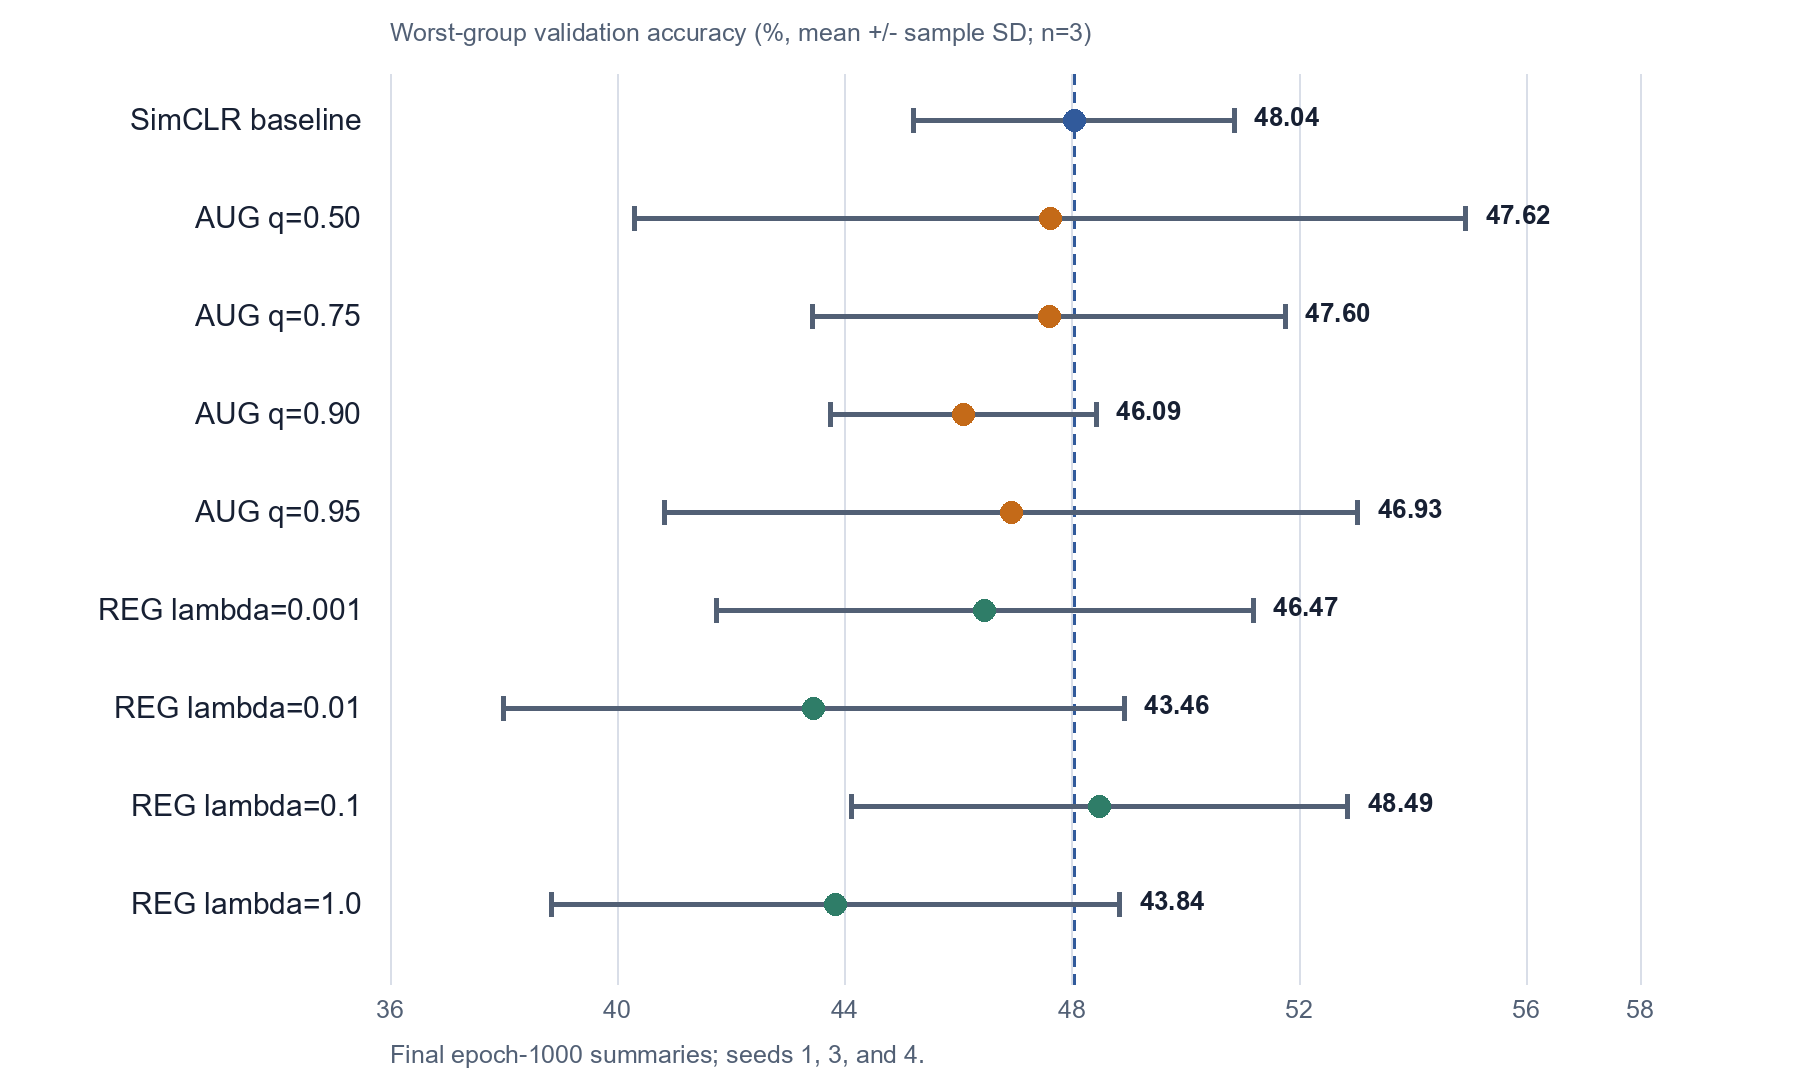
\includegraphics[width=\textwidth]{figures/current_postrepair_wg.png}
\caption{No completed revised method reliably separates from the matched
SimCLR baseline. Error bars are descriptive sample standard deviations, not
confidence intervals; $n=3$ is too small for a strong statistical claim.}
\label{fig:postrepair_wg}
\end{figure}

The completed larger REG weights resolve one open question: $\lambda=0.001$
was indeed almost inactive (final SpLiCE loss near $7\times10^{-6}$), whereas
$\lambda=0.1$ contributes about $6\times10^{-4}$ and can improve individual
seeds. However, the seed-4 regression of $-7.30$ points means that the positive
mean of $+0.45$ points is not a stable effect. At $\lambda=1.0$, the penalty is
roughly $4\times10^{-3}$ and performance worsens overall, suggesting an
intermediate useful scale but no robust setting yet.

The earlier positive AUG result also does not replicate consistently. The most
extreme case is $q=0.50$: it improves seeds 1 and 3 but collapses for seed 4.
Its final seed-4 SSL loss is 0.109 versus 0.026 for the matched baseline,
consistent with the stronger intervention making optimization harder. This is
diagnostic evidence, not proof of the cause.

\noindent\textbf{Current conclusion.} The evidence does not support claiming a
reliable Waterbirds improvement from the present all-components AUG policy or
correlation penalty. It does support the broader research program: the pipeline
can discover interpretable proxies, expose failure modes, and test better ways
to use those proxies. Final test evaluation should remain locked.

\subsection{Strong-Augmentation Components}

\begin{table}[ht]
\centering
\scriptsize
\caption{Current $q=0.75$ augmentation ablation. Values are average / WG
validation accuracy (\%). Seeds 0 and 2 predate the reproducibility repair.}
\label{tab:current_augmentations}
\begin{tabularx}{\textwidth}{l>{\centering\arraybackslash}X
>{\centering\arraybackslash}X>{\centering\arraybackslash}X
>{\centering\arraybackslash}X>{\centering\arraybackslash}X
>{\centering\arraybackslash}X}
\toprule
Strong transform & S0$\dagger$ & S1 & S2$\dagger$ & S3 & S4 & Post-repair WG \\
\midrule
All components & 50.33/39.29 & 54.07/52.08 & 56.16/49.36 & 50.77/43.85 & 52.94/46.87 & $47.60\pm4.16$ \\
Crop only & 52.44/44.80 & 53.72/45.03 & 55.40/46.10 & \texttt{TODO} & \texttt{TODO} & -- ($n=1$) \\
Color jitter only & 48.23/39.08 & 57.80/45.19 & 54.96/44.84 & \texttt{TODO} & \texttt{TODO} & -- ($n=1$) \\
Grayscale only & 53.53/48.52 & 51.66/46.99 & 52.70/38.80 & \texttt{TODO} & \texttt{TODO} & -- ($n=1$) \\
Gaussian blur only & 44.79/34.12 & 51.13/48.91 & 52.49/44.35 & \texttt{TODO} & \texttt{TODO} & -- ($n=1$) \\
\bottomrule
\end{tabularx}
\end{table}

Only the all-components setting has three comparable post-repair seeds, and it
does not beat the matched baseline. The apparent stability of crop in the
mixed-protocol rows cannot yet be treated as confirmation; crop, color jitter,
grayscale, and blur still require post-repair seeds 3 and 4. Seed 1 illustrates
why average accuracy alone is insufficient: color jitter has 57.80\% average
accuracy but only 45.19\% WG accuracy.

The leakage probe remains high for every component run (90.40--92.49\%
average validation accuracy for seed 1). This does not yet support the
stronger claim that the learned representation has stopped encoding the
background. It is possible for target WG accuracy to improve while background
information remains linearly accessible, so both metrics should continue to be
reported.

The repaired diagnostic path is also supported by a direct reproducibility
check: the all-components $q=0.75$ run in this ablation and the independently
submitted $q=0.75$ hyperparameter run produced exactly the same seed-1 result,
54.0701\% average and 52.0850\% WG accuracy, despite diagnostics being enabled
only in the former. Seeds 1, 3, and 4 were all run from commit
\texttt{e1fa215} after the repair; seeds 0 and 2 remain descriptive historical
points only.

\FloatBarrier

\section{Recommended Research Roadmap}

\subsection{Priority 0: Freeze the Current Evidence}

The $q=0.95$ runs and the larger REG weights are now complete. Archive the W\&B
run IDs and this result table, and do not launch final-test jobs. The completed
sweep is sufficient to stop broad sweeps of the current formulation; more seeds
should be reserved for a method that first passes the controls below.

\subsection{Priority 1: Validate the SpLiCE Signal Before Changing the Loss}

The selected set contains plausible background concepts (\texttt{forest},
\texttt{lake}, \texttt{pond}) but also ambiguous or target-related concepts
(\texttt{raven}, \texttt{whale}, \texttt{snorkeling}). Moreover, the current
discovery score uses absolute background differences. It penalizes differences
in \emph{magnitude} across target classes but does not explicitly reject a
concept whose signed background effect reverses between bird classes. This is a
high-value methodological check.

Run the following inexpensive ablations before designing a more complex model:
\begin{enumerate}
    \item compare top-$K\in\{3,5,10,20\}$ and merge near-duplicate vocabulary
    items such as \texttt{forest}/\texttt{forests};
    \item require consistent signed background direction across target classes,
    or rank concepts by a small cross-validated background probe conditioned on
    target;
    \item compare the automatic list with a curated background-only list;
    \item add random routing and shuffled SpLiCE-score controls at the same
    routed fraction. A gain over standard SimCLR but not over these controls
    would be an augmentation-strength effect, not evidence for semantic routing.
\end{enumerate}

\subsection{Priority 2: Make the Contrastive Objective Concept-Aware}

The preferred new method is a \textbf{concept-conditioned contrastive
objective}. SimCLR currently treats only two views of the same image as a
positive pair. Use SpLiCE to construct additional hard positives: images with
the same target label but different background-concept profiles. Their
representations should be pulled together, while images from different target
classes remain negatives. This directly encodes the desired geometry---same
bird class, different background---instead of hoping that a generic strong
augmentation removes the correct feature. It is closely related to supervised
contrastive learning \cite{khosla2020supcon}, but with positive selection
conditioned on concept dissimilarity.

A minimal objective is
\[
\mathcal L = \mathcal L_{\mathrm{SimCLR}}
+ \alpha\,\mathcal L_{\mathrm{cross\mbox{-}background\ positive}},
\]
where the additional positive for image $i$ has the same $y$ but low cosine
similarity between SpLiCE vectors $c_i$ and $c_j$. Start with
$\alpha\in\{0.05,0.1,0.25\}$ and report both target WG accuracy and spurious
probe accuracy. This method uses target labels during pretraining and must be
described as label-conditioned or weakly supervised, just like the current REG
objective.

If a strictly label-free claim is required, a weaker alternative is to create a
counterfactual second view of the \emph{same} image using background-specific
masks or generation, and keep the ordinary same-image InfoNCE pair. Another
label-free direction is learning-speed-aware sampling, which has been proposed
for robust SSL under spurious correlations \cite{zhu2023lassl}.

\subsection{Priority 3: Compare Better Invariance Losses}

The current squared Pearson-correlation penalty only removes linear dependence
and its scale depends strongly on averaging over all feature--concept pairs.
Three controlled alternatives are worth testing:
\begin{enumerate}
    \item \textbf{Normalized cross-covariance/HSIC penalty:} whiten or
    variance-normalize $h$ and $c$ before penalizing dependence; tune by the
    observed ratio $\mathcal L_{\mathrm{concept}}/\mathcal L_{\mathrm{SSL}}$
    rather than raw $\lambda$.
    \item \textbf{Conditional adversarial removal:} train a small head to
    predict the SpLiCE vector or background attribute from $h$ and reverse its
    gradient, conditioned on target. This can remove nonlinear leakage but is
    less stable and needs a careful adversary-capacity sweep.
    \item \textbf{Late-layer intervention:} apply the dependence penalty or
    pruning only to later encoder blocks. Prior robust-SSL work reports that
    targeted feature-space interventions can outperform generic resampling or
    view changes \cite{hamidieh2024views}.
\end{enumerate}

\subsection{Experiment Matrix and Stop Rules}

\begin{table}[ht]
\centering
\small
\caption{Prioritized experiments after the current runs finish.}
\begin{tabularx}{\textwidth}{p{0.25\textwidth}p{0.33\textwidth}X}
\toprule
Experiment & Question answered & Continue only if \\
\midrule
Shuffled/random routing & Does SpLiCE semantics matter beyond stronger
augmentation? & Semantic routing beats both controls in paired WG. \\
Signed concept selection and top-$K$ & Is the proxy specific and stable? & The
list is qualitatively background-related and target-conditioned background
prediction improves. \\
Single augmentation components, seeds 3/4 & Is one transformation safer than
the all-components policy? & At least two post-repair seeds improve WG without
large average-accuracy loss. \\
Concept-conditioned positives & Does direct cross-background alignment improve
the geometry? & Mean paired WG improves, seed signs are mostly consistent, and
spurious leakage decreases. \\
Adversarial or normalized dependence loss & Is linear correlation too weak? &
Leakage falls without representation collapse or target-WG regression. \\
Transfer to SpurCIFAR10/CelebA & Does the method generalize? & Waterbirds first
passes the controls with a frozen hyperparameter rule. \\
\bottomrule
\end{tabularx}
\end{table}

\section{Claim to Make at the Meeting}

The defensible message is: \emph{I implemented and repaired a complete
concept-guided robust-SSL evaluation pipeline. The initial positive result did
not survive the stricter paired-seed protocol, which revealed strong seed
sensitivity and weaknesses in concept selection and loss scaling. The project
has therefore progressed from a proof-of-concept to a falsifiable research
program. The next high-information experiment is not ``more of the same'', but
to verify that the semantic routing signal matters and then place that signal
directly into contrastive pair construction.}

\section{Limitations}

There are only three comparable post-repair seeds, and no revised configuration
has been evaluated on the held-out test split. Waterbirds metadata are used both
for concept discovery and for
label-conditioned regularization, so the current method is not fully
self-supervised. The leakage probe is linear and cannot rule out nonlinear
background information. Finally, W\&B final-ten averages summarize noisy
training curves but are not confidence intervals.

\FloatBarrier
\appendix

\section{Preliminary Legacy Results (Scalar Control)}

``Legacy'' denotes a materially different experimental definition, not merely
an earlier software revision. Table~\ref{tab:legacy_protocol} states the main
differences. In particular, the old and current scores should not be read as a
before/after benchmark of the same method.

\begin{table}[ht]
\centering
\small
\caption{Why the legacy and revised experiments answer different questions.}
\label{tab:legacy_protocol}
\begin{tabularx}{\textwidth}{lXX}
\toprule
Aspect & Legacy protocol & Revised protocol \\
\midrule
Concept selection & Manually named concepts & Top concepts selected automatically from training metadata \\
AUG routing & Fixed absolute threshold $\tau$ & Training-score quantile $q$, robust to score scale \\
AUG views & Two strong views & Standard view paired with a strong view \\
REG objective & One global scalar correlation & Target-conditioned feature--concept correlation matrix \\
Model selection & Test results observed during exploration & Validation-only selection; final test held back \\
Diagnostics & Shared training-loader random state & Isolated deterministic loader and preserved RNG state \\
\bottomrule
\end{tabularx}
\end{table}

The legacy numbers can be higher without showing that the revised design is
worse. First, repeatedly observing the test split while trying configurations
introduces selection bias: the best observed test result is likely to include
favourable noise. Second, two strong views and a manually chosen absolute
threshold define a more aggressive, dataset-specific intervention than the
current method. Third, the revised REG objective removes a full conditional
correlation structure rather than optimizing the earlier scalar proxy. The
revision is intended to make the hypothesis test reproducible, target-aware,
and transferable; it is not guaranteed to increase accuracy. A fair performance
comparison requires selecting each method on validation data and evaluating it
once on an untouched test split.

\begin{table}[ht]
\centering
\small
\caption{Compact summary of the legacy scalar-control sweep over three seeds
(mean $\pm$ sample standard deviation, \%).}
\label{tab:results}
\begin{tabular}{llcc}
\toprule
Method & Parameter & Average accuracy & WG accuracy \\
\midrule
Baseline SSL & -- & $52.30\pm5.32$ & $44.45\pm5.34$ \\
SpLiCE-AUG & $\tau=0.03$ & $56.64\pm1.35$ & $51.41\pm1.99$ \\
SpLiCE-AUG & $\tau=0.05$ & $53.66\pm0.88$ & $47.68\pm6.47$ \\
SpLiCE-AUG & $\tau=0.085$ & $53.81\pm2.22$ & $48.74\pm1.87$ \\
SpLiCE-AUG & $\tau=0.10$ & $53.40\pm3.20$ & $46.99\pm5.70$ \\
SpLiCE-REG & $\lambda=0.0001$ & $49.63\pm1.35$ & $41.53\pm1.29$ \\
SpLiCE-REG & $\lambda=0.0005$ & $53.12\pm2.81$ & $46.27\pm7.82$ \\
SpLiCE-REG & $\lambda=0.001$ & $54.15\pm4.65$ & $48.03\pm5.95$ \\
SpLiCE-REG & $\lambda=0.005$ & $52.20\pm0.23$ & $45.21\pm3.19$ \\
\bottomrule
\end{tabular}
\end{table}

The strongest legacy result is SpLiCE-AUG with $\tau=0.03$, improving mean WG
accuracy from 44.45\% to 51.41\%. This is useful evidence that concept-guided
augmentation can help, but it remains exploratory evidence under the legacy
protocol rather than a confirmatory estimate for the revised method.

\begin{table}[ht]
\centering
\small
\caption{Legacy component ablations, summarized over three seeds. Only WG
accuracy is shown because it is the primary robustness metric.}
\label{tab:legacy_augmentation_components}
\begin{tabular}{llc}
\toprule
Dataset & Strong component & WG mean $\pm$ std. \\
\midrule
Waterbirds & Crop & $46.17\pm5.76$ \\
Waterbirds & Color jitter & $47.73\pm1.74$ \\
Waterbirds & Grayscale & $47.76\pm7.95$ \\
Waterbirds & Gaussian blur & $44.61\pm1.19$ \\
Waterbirds & All components & $50.47\pm1.76$ \\
\midrule
SpurCIFAR10 & Crop & $30.24\pm2.37$ \\
SpurCIFAR10 & Color jitter & $29.88\pm7.55$ \\
SpurCIFAR10 & Grayscale & $26.33\pm5.34$ \\
SpurCIFAR10 & Gaussian blur & $26.52\pm5.69$ \\
SpurCIFAR10 & All components & $30.42\pm3.84$ \\
\bottomrule
\end{tabular}
\end{table}

These component runs used the strong variants crop scale $(0.08,1.0)$, color
jitter $(0.8,0.8,0.8,0.2)$ with probability 0.9, grayscale probability 0.3,
and Gaussian blur probability 0.5. Their seed dependence motivated the current
component sweep; they do not identify one universally best transform.

\FloatBarrier

\section{SpLiCE Concept Scoring and Regularization Formulas}

Let \(c_k(x)\) denote the SpLiCE weight of concept \(k\) for image \(x\).
For Waterbirds, each image has a target label $ y \in \{0,1\}$
and a spurious/background attribute $ s \in \{0,1\}. $
For each concept \(k\), the discovery script first computes the mean SpLiCE concept weight inside each metadata group:
\[
\mu_k(s,y)
=
\mathbb{E}\left[c_k(x)\mid s(x)=s,\ y(x)=y\right].
\]
Thus, for the binary Waterbirds setting, each concept has four group means:
\[
\mu_k(0,0),\quad
\mu_k(1,0),\quad
\mu_k(0,1),\quad
\mu_k(1,1).
\]

\subsection{Spurious Effect}

The spurious effect measures how much concept \texttt{k} changes when the background \texttt{s} changes, while keeping the bird label \texttt{y} fixed:
\[
\Delta^{\mathrm{spur}}_k(y)
=
\mu_k(1,y)-\mu_k(0,y).
\]
The reported spurious value is the average absolute effect across target classes:
\[
\mathrm{Spurious}_k
=
\frac{1}{2}
\left(
\left|\mu_k(1,0)-\mu_k(0,0)\right|
+
\left|\mu_k(1,1)-\mu_k(0,1)\right|
\right).
\]
A high spurious value means that the concept is strongly related to spurious feature, which is a desirable behavior in our case.
\subsection{Target Effect}

The target effect measures how much concept \texttt{k} changes when the bird label \texttt{y} changes, while keeping the background \texttt{s} fixed:
\[
\Delta^{\mathrm{target}}_k(s)
=
\mu_k(s,1)-\mu_k(s,0).
\]
The reported target value is:
\[
\mathrm{Target}_k
=
\frac{1}{2}
\left(
\left|\mu_k(0,1)-\mu_k(0,0)\right|
+
\left|\mu_k(1,1)-\mu_k(1,0)\right|
\right).
\]
A high target value means that the concept is strongly related to the actual bird class, which is not desirable when searching for background-related concepts.

\subsection{Instability}

The instability term measures whether the \emph{magnitude} of the spurious
effect is consistent across target classes. Define
\[
 a_k = \left|\mu_k(1,0)-\mu_k(0,0)\right|,
\]
\[
 b_k = \left|\mu_k(1,1)-\mu_k(0,1)\right|.
\]
The script computes the standard deviation of these two values:
\[
\mathrm{Instability}_k
=
\sqrt{
\frac{1}{2}
\left[
(a_k-\bar{d}_k)^2
+
(b_k-\bar{d}_k)^2
\right]
},
\]
where
\[
\bar{d}_k
=
\frac{a_k+b_k}{2}.
\]
Low instability means that the concept behaves similarly for both bird classes. High instability means that the concept only behaves like a spurious concept for one target class.

\subsection{Final Discovery Score}

The final concept discovery score is computed as
\[
\mathrm{Score}_k
=
\mathrm{Spurious}_k
-
\lambda_y \mathrm{Target}_k
-
\lambda_{\mathrm{inst}} \mathrm{Instability}_k.
\]
Here, \(\lambda_y\) is controlled by \texttt{--label\_penalty}, and
\(\lambda_{\mathrm{inst}}\) is controlled by \texttt{--instability\_penalty}.
By default, both values are equal to \(1.0\), so the default formula is
\[
\mathrm{Score}_k
=
\mathrm{Spurious}_k
-
\mathrm{Target}_k
-
\mathrm{Instability}_k.
\]
Therefore, the script ranks concepts highly when they have a strong spurious effect, a weak target effect, and low instability.

\paragraph{Important discovery caveat.}
Because the pairwise effects above use absolute differences, two target classes
can have equally large but oppositely signed background effects and still receive
zero instability penalty. A direction-consistency term should therefore be
tested before treating the selected top-$K$ as a reliable background proxy.

\subsection{Correlation Regularization Penalty}

In the revised \texttt{corr\_reg} mode, SpLiCE retains the selected concept
vector $c_i\in\mathbb{R}^{K}_{\geq0}$ for each training image, with $K=10$ in
the current experiments. The SSL encoder produces
\[
h_i = f_{\theta}(x_i) \in \mathbb{R}^d.
\]
Because background and target are correlated in the biased training set, the
default loss first centres embeddings and concept vectors separately within
each target class $B_y=\{i:y_i=y\}$:
\[
\widetilde h_i=h_i-\frac{1}{|B_{y_i}|}\sum_{j\in B_{y_i}}h_j,
\qquad
\widetilde c_i=c_i-\frac{1}{|B_{y_i}|}\sum_{j\in B_{y_i}}c_j.
\]
It then computes every embedding--concept correlation
\[
R_{jk}=
\frac{\sum_i \widetilde h_{ij}\widetilde c_{ik}}
{\sqrt{\sum_i\widetilde h_{ij}^{2}}
 \sqrt{\sum_i\widetilde c_{ik}^{2}}+\epsilon}.
\]
The revised vector-valued penalty is
\[
\mathcal{L}_{\mathrm{SpLiCE}}
=
\lambda_{\mathrm{SpLiCE}}
\frac{1}{dK}
\sum_{j=1}^{d}\sum_{k=1}^{K}R_{jk}^2.
\]
Here, \(\lambda_{\mathrm{SpLiCE}}\) is the regularization weight controlled by
\texttt{--splice\_weight}. The full SSL training objective becomes
\[
\mathcal{L}
=
\mathcal{L}_{\mathrm{SimCLR}}
+
\mathcal{L}_{\mathrm{SpLiCE}}.
\]
Thus the regularizer discourages any linear SSL feature from encoding any of
the selected SpLiCE coordinates \emph{within a fixed target class}. It does not
identify a one-to-one ``background neuron'', and because it uses target labels
inside the SSL loss it must be described as label-conditioned rather than fully
label-free.

\subsection{Score Distribution in Concept Summarization}

After concept discovery, we select a set of concepts \(C\), for example
\[
C =
\{
\texttt{bamboo},
\texttt{forests},
\texttt{whale},
\texttt{rainforest},
\texttt{raven},
\texttt{forest},
\texttt{seascape},
\texttt{lake},
\texttt{snorkeling},
\texttt{pond}
\}.
\]
For every image \(x_i\), the summarization script computes one scalar score
\(r_i\) from the selected concept weights.

If \texttt{--splice\_score\_reduction max} is used, then
\[
r_i
=
\max_{k \in C} c_k(x_i).
\]
The score distribution is the empirical distribution of these image-level
scores:
\[
\{r_1,r_2,\ldots,r_n\}.
\]
The reported values such as the median, \(p75\), \(p90\), and \(p95\) are
percentiles of this distribution.

For a threshold \(\tau\), the script reports the number of images whose score is
above the threshold:
\[
N_{\tau}
=
\sum_{i=1}^{n}
\mathbf{1}[r_i \geq \tau],
\]
and the corresponding fraction:
\[
F_{\tau}
=
\frac{1}{n}
\sum_{i=1}^{n}
\mathbf{1}[r_i \geq \tau].
\]
This tells us how many training images will be treated as high SpLiCE-score
examples. In the augmentation method, images with
\[
r_i \geq \tau
\]
receive the stronger augmentation transform.


\section{Reproduction and Next Experiment Commands}

\paragraph{1. Standalone concept discovery (optional audit).}
The following standalone command is useful for auditing the selected concepts:

\begin{verbatim}
python tools/discover_splice_spurious_concepts.py \
  --dataset waterbirds \
  --data_folder ./datasets \
  --split train \
  --out_path outputs/waterbirds_splice_concepts.json \
  --top_k 10
\end{verbatim}

In one run, the top-10 concepts were:
\begin{verbatim}
8305 bamboo      score=0.010589 spurious=0.016997 target=0.003204 instability=0.003204
2908 forests     score=0.004767 spurious=0.006347 target=0.000822 instability=0.000758
6265 whale       score=0.001928 spurious=0.002307 target=0.000189 instability=0.000189
4730 rainforest  score=0.001892 spurious=0.003017 target=0.000565 instability=0.000560
591  raven       score=0.001616 spurious=0.002540 target=0.000715 instability=0.000209
9479 forest      score=0.001492 spurious=0.002912 target=0.000710 instability=0.000710
4623 seascape    score=0.001484 spurious=0.002110 target=0.000313 instability=0.000313
9411 lake        score=0.001310 spurious=0.001343 target=0.000017 instability=0.000017
1158 snorkeling  score=0.001178 spurious=0.001433 target=0.000143 instability=0.000112
8045 pond        score=0.001129 spurious=0.001685 target=0.000278 instability=0.000278
\end{verbatim}

Here, \texttt{spurious} measures how much the concept changes with the
background attribute after conditioning on the bird label. \texttt{target}
measures how much the same concept changes with the bird label after
conditioning on the background. \texttt{instability} measures whether the
spurious effect is inconsistent across target classes. The final
\texttt{score} is the ranking value used by the script: high spurious effect is
rewarded, while target-label effect and instability are penalized. Therefore,
higher-score concepts are better candidates for representing the spurious
background signal.

\paragraph{2. Summarize selected concept scores.}
After selecting candidate concepts, the next step is to check the distribution
of their SpLiCE scores across the training split. This helps choose a threshold
for the augmentation method.

\begin{verbatim}
python tools/summarize_splice_scores.py \
  --data_folder ./datasets \
  --split train \
  --splice_concepts "bamboo,forests,whale,rainforest,raven,forest,seascape,lake,
                     snorkeling,pond" \
  --splice_score_reduction max \
  --out_path outputs/waterbirds_splice_score_summary.json
\end{verbatim}

The output first resolves each concept to its vocabulary index, then reports the
score distribution over all images in the split. The percentiles summarize how
large the selected-concept score usually is, while the threshold counts show how
many images would be treated as high-score examples for each candidate
threshold. For example, in the shown run, threshold 0.085 selects 1007 training
images, or about 21.0\% of the split.

\paragraph{3. Transfer the protocol to SpurCIFAR10.}
The same arrays now accept \texttt{DATASET} as an exported variable and choose
\texttt{resnet18} automatically for 32$\times$32 inputs. Dataset-level concept
discovery and caches remain separate because the dataset name is included in
their paths and fingerprints.

\begin{verbatim}
sbatch --job-name=SpurCIFAR10_SpLiCE_sweep \
  --export=ALL,DATASET=spur_cifar10,SEED=0 \
  waterbirds_SpLiCE_hyperparameter_array.sbatch

sbatch --job-name=SpurCIFAR10_SpLiCE_aug \
  --export=ALL,DATASET=spur_cifar10,SEED=0 \
  waterbirds_Augmentation_array.sbatch
\end{verbatim}

The existing case statement fixes $q$ and $\lambda$ for each array index, so
exporting \texttt{SPLICE\_SCORE\_QUANTILE} or \texttt{SPLICE\_WEIGHT} currently
does not override them. Finer sweeps require new case entries or changing those
assignments to environment-default form. The most useful controls after the
replication seeds are: (i) global strong augmentation applied to a random or all
images, to distinguish SpLiCE routing from augmentation strength; (ii) shuffled
SpLiCE scores, to test whether semantic targeting matters; (iii) conditional
versus unconditional REG; (iv) combined AUG+REG; and (v) sparse SpLiCE-CBM
representation/probe interventions. Final test jobs should be launched only
after this validation stage and must use the explicit \texttt{--final\_test}
guard.

\begin{thebibliography}{9}

\bibitem{bhalla2024splice}
U. Bhalla, A. Oesterling, S. Srinivas, F. P. Calmon, and H. Lakkaraju.
\newblock Interpreting CLIP with Sparse Linear Concept Embeddings (SpLiCE).
\newblock \emph{NeurIPS}, 2024. \url{https://arxiv.org/abs/2402.10376}.

\bibitem{chen2020simclr}
T. Chen, S. Kornblith, M. Norouzi, and G. Hinton.
\newblock A Simple Framework for Contrastive Learning of Visual Representations.
\newblock \emph{ICML}, 2020.
\url{https://proceedings.mlr.press/v119/chen20j.html}.

\bibitem{khosla2020supcon}
P. Khosla et al.
\newblock Supervised Contrastive Learning.
\newblock \emph{NeurIPS}, 2020.
\url{https://proceedings.neurips.cc/paper/2020/hash/d89a66c7c80a29b1bdbab0f2a1a94af8-Abstract.html}.

\bibitem{hamidieh2024views}
K. Hamidieh, H. Zhang, S. Sankaranarayanan, and M. Ghassemi.
\newblock Views Can Be Deceiving: Improved SSL Through Feature Space Augmentation.
\newblock \emph{ICLR}, 2024.
\url{https://proceedings.iclr.cc/paper_files/paper/2024/file/9c7900fac04a701cbed83256b76dbaa3-Paper-Conference.pdf}.

\bibitem{zhu2023lassl}
W. Zhu, S. Liu, C. Fernandez-Granda, and N. Razavian.
\newblock Making Self-supervised Learning Robust to Spurious Correlation via
Learning-speed Aware Sampling.
\newblock NeurIPS 2023 Workshop on Self-Supervised Learning.
\url{https://arxiv.org/abs/2311.16361}.

\end{thebibliography}

\end{document}
